\documentclass[11pt]{article}\usepackage[]{graphicx}\usepackage[]{color}
% maxwidth is the original width if it is less than linewidth
% otherwise use linewidth (to make sure the graphics do not exceed the margin)
\makeatletter
\def\maxwidth{ %
  \ifdim\Gin@nat@width>\linewidth
    \linewidth
  \else
    \Gin@nat@width
  \fi
}
\makeatother

\definecolor{fgcolor}{rgb}{0.345, 0.345, 0.345}
\newcommand{\hlnum}[1]{\textcolor[rgb]{0.686,0.059,0.569}{#1}}%
\newcommand{\hlstr}[1]{\textcolor[rgb]{0.192,0.494,0.8}{#1}}%
\newcommand{\hlcom}[1]{\textcolor[rgb]{0.678,0.584,0.686}{\textit{#1}}}%
\newcommand{\hlopt}[1]{\textcolor[rgb]{0,0,0}{#1}}%
\newcommand{\hlstd}[1]{\textcolor[rgb]{0.345,0.345,0.345}{#1}}%
\newcommand{\hlkwa}[1]{\textcolor[rgb]{0.161,0.373,0.58}{\textbf{#1}}}%
\newcommand{\hlkwb}[1]{\textcolor[rgb]{0.69,0.353,0.396}{#1}}%
\newcommand{\hlkwc}[1]{\textcolor[rgb]{0.333,0.667,0.333}{#1}}%
\newcommand{\hlkwd}[1]{\textcolor[rgb]{0.737,0.353,0.396}{\textbf{#1}}}%
\let\hlipl\hlkwb

\usepackage{framed}
\makeatletter
\newenvironment{kframe}{%
 \def\at@end@of@kframe{}%
 \ifinner\ifhmode%
  \def\at@end@of@kframe{\end{minipage}}%
  \begin{minipage}{\columnwidth}%
 \fi\fi%
 \def\FrameCommand##1{\hskip\@totalleftmargin \hskip-\fboxsep
 \colorbox{shadecolor}{##1}\hskip-\fboxsep
     % There is no \\@totalrightmargin, so:
     \hskip-\linewidth \hskip-\@totalleftmargin \hskip\columnwidth}%
 \MakeFramed {\advance\hsize-\width
   \@totalleftmargin\z@ \linewidth\hsize
   \@setminipage}}%
 {\par\unskip\endMakeFramed%
 \at@end@of@kframe}
\makeatother

\definecolor{shadecolor}{rgb}{.97, .97, .97}
\definecolor{messagecolor}{rgb}{0, 0, 0}
\definecolor{warningcolor}{rgb}{1, 0, 1}
\definecolor{errorcolor}{rgb}{1, 0, 0}
\newenvironment{knitrout}{}{} % an empty environment to be redefined in TeX

\usepackage{alltt}
%Required: You must have these
\usepackage{graphicx}
\usepackage{tabularx}
\usepackage{natbib}
\usepackage{pdflscape}
\usepackage{array}
\usepackage{authblk}
\usepackage{gensymb}
\usepackage{amsmath}
\usepackage{rotating}

%\usepackage[backend=bibtex]{biblatex}
\usepackage[small]{caption}

\setkeys{Gin}{width=0.8\textwidth}
\setlength{\captionmargin}{30pt}
\setlength{\abovecaptionskip}{10pt}
\setlength{\belowcaptionskip}{10pt}

 \topmargin -1.5cm 
 \oddsidemargin -0.04cm 
 \evensidemargin -0.04cm 
 \textwidth 16.59cm
 \textheight 21.94cm 
 \parskip 7.2pt 
\renewcommand{\baselinestretch}{1.6} 	
\parindent 0pt
\usepackage{setspace}
\usepackage{lineno}

\bibliographystyle{..//refs/styles/besjournals.bst}
\usepackage{xr-hyper}
\usepackage{hyperref}
%\externaldocument{SUPP_FLS_flobud}

\title{Differences in germination responses to environmental variation among species suggests the potential for strong seasonal priory effects in herbaceous forest communities}
\date{}
\author{}
\IfFileExists{upquote.sty}{\usepackage{upquote}}{}
\begin{document}
\maketitle
\linenumbers
\section{Introduction}

\noindent A core task of community ecology is explain patterns of community assembly across a diversity of ecosystems \citep{Weiher:2011aa}. A central tenet of community assembly theory is that the order of arrival of species to a community mediates inter-specific interactions and can dictate the trajectory of community structure in the long term \citep{Fukami2015}. These historical contingencies, known as priority effects, have been shown to alter the structure and function of communities, even driving communities to alternate stable states \citep{Fukami2011}.\\

\noindent In many ecosystems across the temperate regions of the globe, plant communities must re-assemble each spring after a period of winter dormancy. In these communities, priority effects are largely the product of the rate at which dormant plants and seeds respond to their environment and resume growth or germinate when favorable conditions return\citep{Rudolf:2019aa}, rather than the the timing of the arrival of these propagules, which in many cases occurs in the autumn prior to the dormant season \citep{Howe:1982aa,Baskin:1988aa}.

\noindent% Like traditional historical contigencies, 
The importance of this subcategory of priority effects, known as seasonal priority effects SPEs \citep{Wainwright_2011} or short-term priory \citep{Young:2017aa} to seasonal assembly depends on the magnitude of interspecific differences in germination rate responses to environment. If species have sufficiently different germination rate responses to their environment than the strength of priority effects should vary over time which, can lead to inter-specific coexistence via the storage effect \citep{Towers:2020aa}.\\%SPEs can operate though niche preemption, in which the species with earlier activity reduces the amount of resources available for species with more delayed activity, or niche modification, in which earlier actors modify the environment, determining the growth conditions that later acting species will experience \citep{Fukami2015}. \\

\noindent These dynamics have been primarily demonstrated through experiments that stagger the planting time of competing species to evaluate whether SPEs mechanistically effect competitive outcomes among species \citep{Young:2017aa,Letten:2018aa}. A recent review paper by \citet{Weidlich:2020aa} reported that of 42 out of the 43 studies they evaluated found evidence for priority effects, and 18 of those studies (42\%) included planting interval treatments of less than 1 month, which can approximate the time scale of SPEs. \\

\noident While this evidence suggests priority effects may be important in regulating community interactions, it is unclear to what extent these patterns are broadly generalizable. First, almost all mechanistic tests for SPEs to date have been performed using species from temperate grasslands \citep{Weidlich:2020aa}, whose germination behavior may differ substantially from taxa in other habitats \citep{Tudela-Isanta:2018aa}. Second, it is largely unknown if the magnitude temporal lags applied in staggered planting experiments can be generated under nature conditions. In most natural systems, the timing of germination is dictated by environmental cues---temperature (both cool stratification temperatures to break dormancy and warm incubation temperatures to stimulate germination), moisture and light availability \citep{Bewley1997,Fenner2000}. Shared cue use may constrain differences in germination rate responses among species if species utilize cues in the same way. Broadly characterizing the importance of SPEs in community assembly will require quantifying the magnitude of differences in germination rate responses among a diversity of species across a variety of habitats.\\

\noindent This effort is particularly important and timely as anthropogenic climatic change is altering the germination environments of species across the globe \citep{Walck2011}.  Such sustained alterations to environmental cues have potential to disrupt SPEs, shifting balances of species' interactions, and impacting population demography, community composition and ecosystem functions.\\ 

In this study, we quantified the differences in germination rate responses to temperature for a suite of herbaceous species found in temperate forests with full-factorial growth-chamber experiment in which we manipulated the duration of stratification duration and incubation temperatures to test whether variation in germination order generated by environmental variability can be on the same magnitude as planting intervals from staggered planting experiments to expect strong priory effects.

\section*{Methods}
\subsection*{Species}
\begin{enumerate}
\item Mix of field and forest species because seed bank of forest is often old field
\item Mix of dormancy classes
\end{enumerate}
\subsection{Experimental Methods}
\subsection{Data analysis}
I think we're going with the survival model. I'll just mention survival models assume everything germination, which is a bad assumption so we decided anything that the t50 was greater than 30 days (or other) did not germination higher than that.

\subsection{extension of literature review}
\begin{enumerate}
\item search terms, how many studies in Young 2017
\item how many we added
\end{enumerate}

\section*{Results}
\begin{enumerate}
\item table 1: Matrix of species differences under climate change and regular conditions
\item figure 1: mu plots, shape
\item plot of germination ranks under each scenario
\item 3d plots with t50, temperature and stratification for each species?
\item Supp table of lit review with quantification of responses (x out of y studies found priority effects with germination differences of <7 days, 7-21 days etc)
\end{enumerate}


\section*{Discussion}
\begin{itemize}
\item Yes, it seem like the differences are big enough to alter germination rank
\item Next, we have to investigate if these differences drive performance differences (priority effects)
\item Our study didn't include risks to early germination--stabilizing selection on germination time.
\item Germination may be less important in forest systems But germination may become more important as the need to migrate or disturbance regimes change.
\item Population differences, maternal effects etc not accounted for.
\item in forest germination compete with tamers not just other seeds.
\item These result should fit into larger demography models that include survival, reproductive output etc.
\end{itemize}
\bibliography{..//refs/germination.bib} 
\section*{Figures}
\begin{figure}[h!]
    \centering
 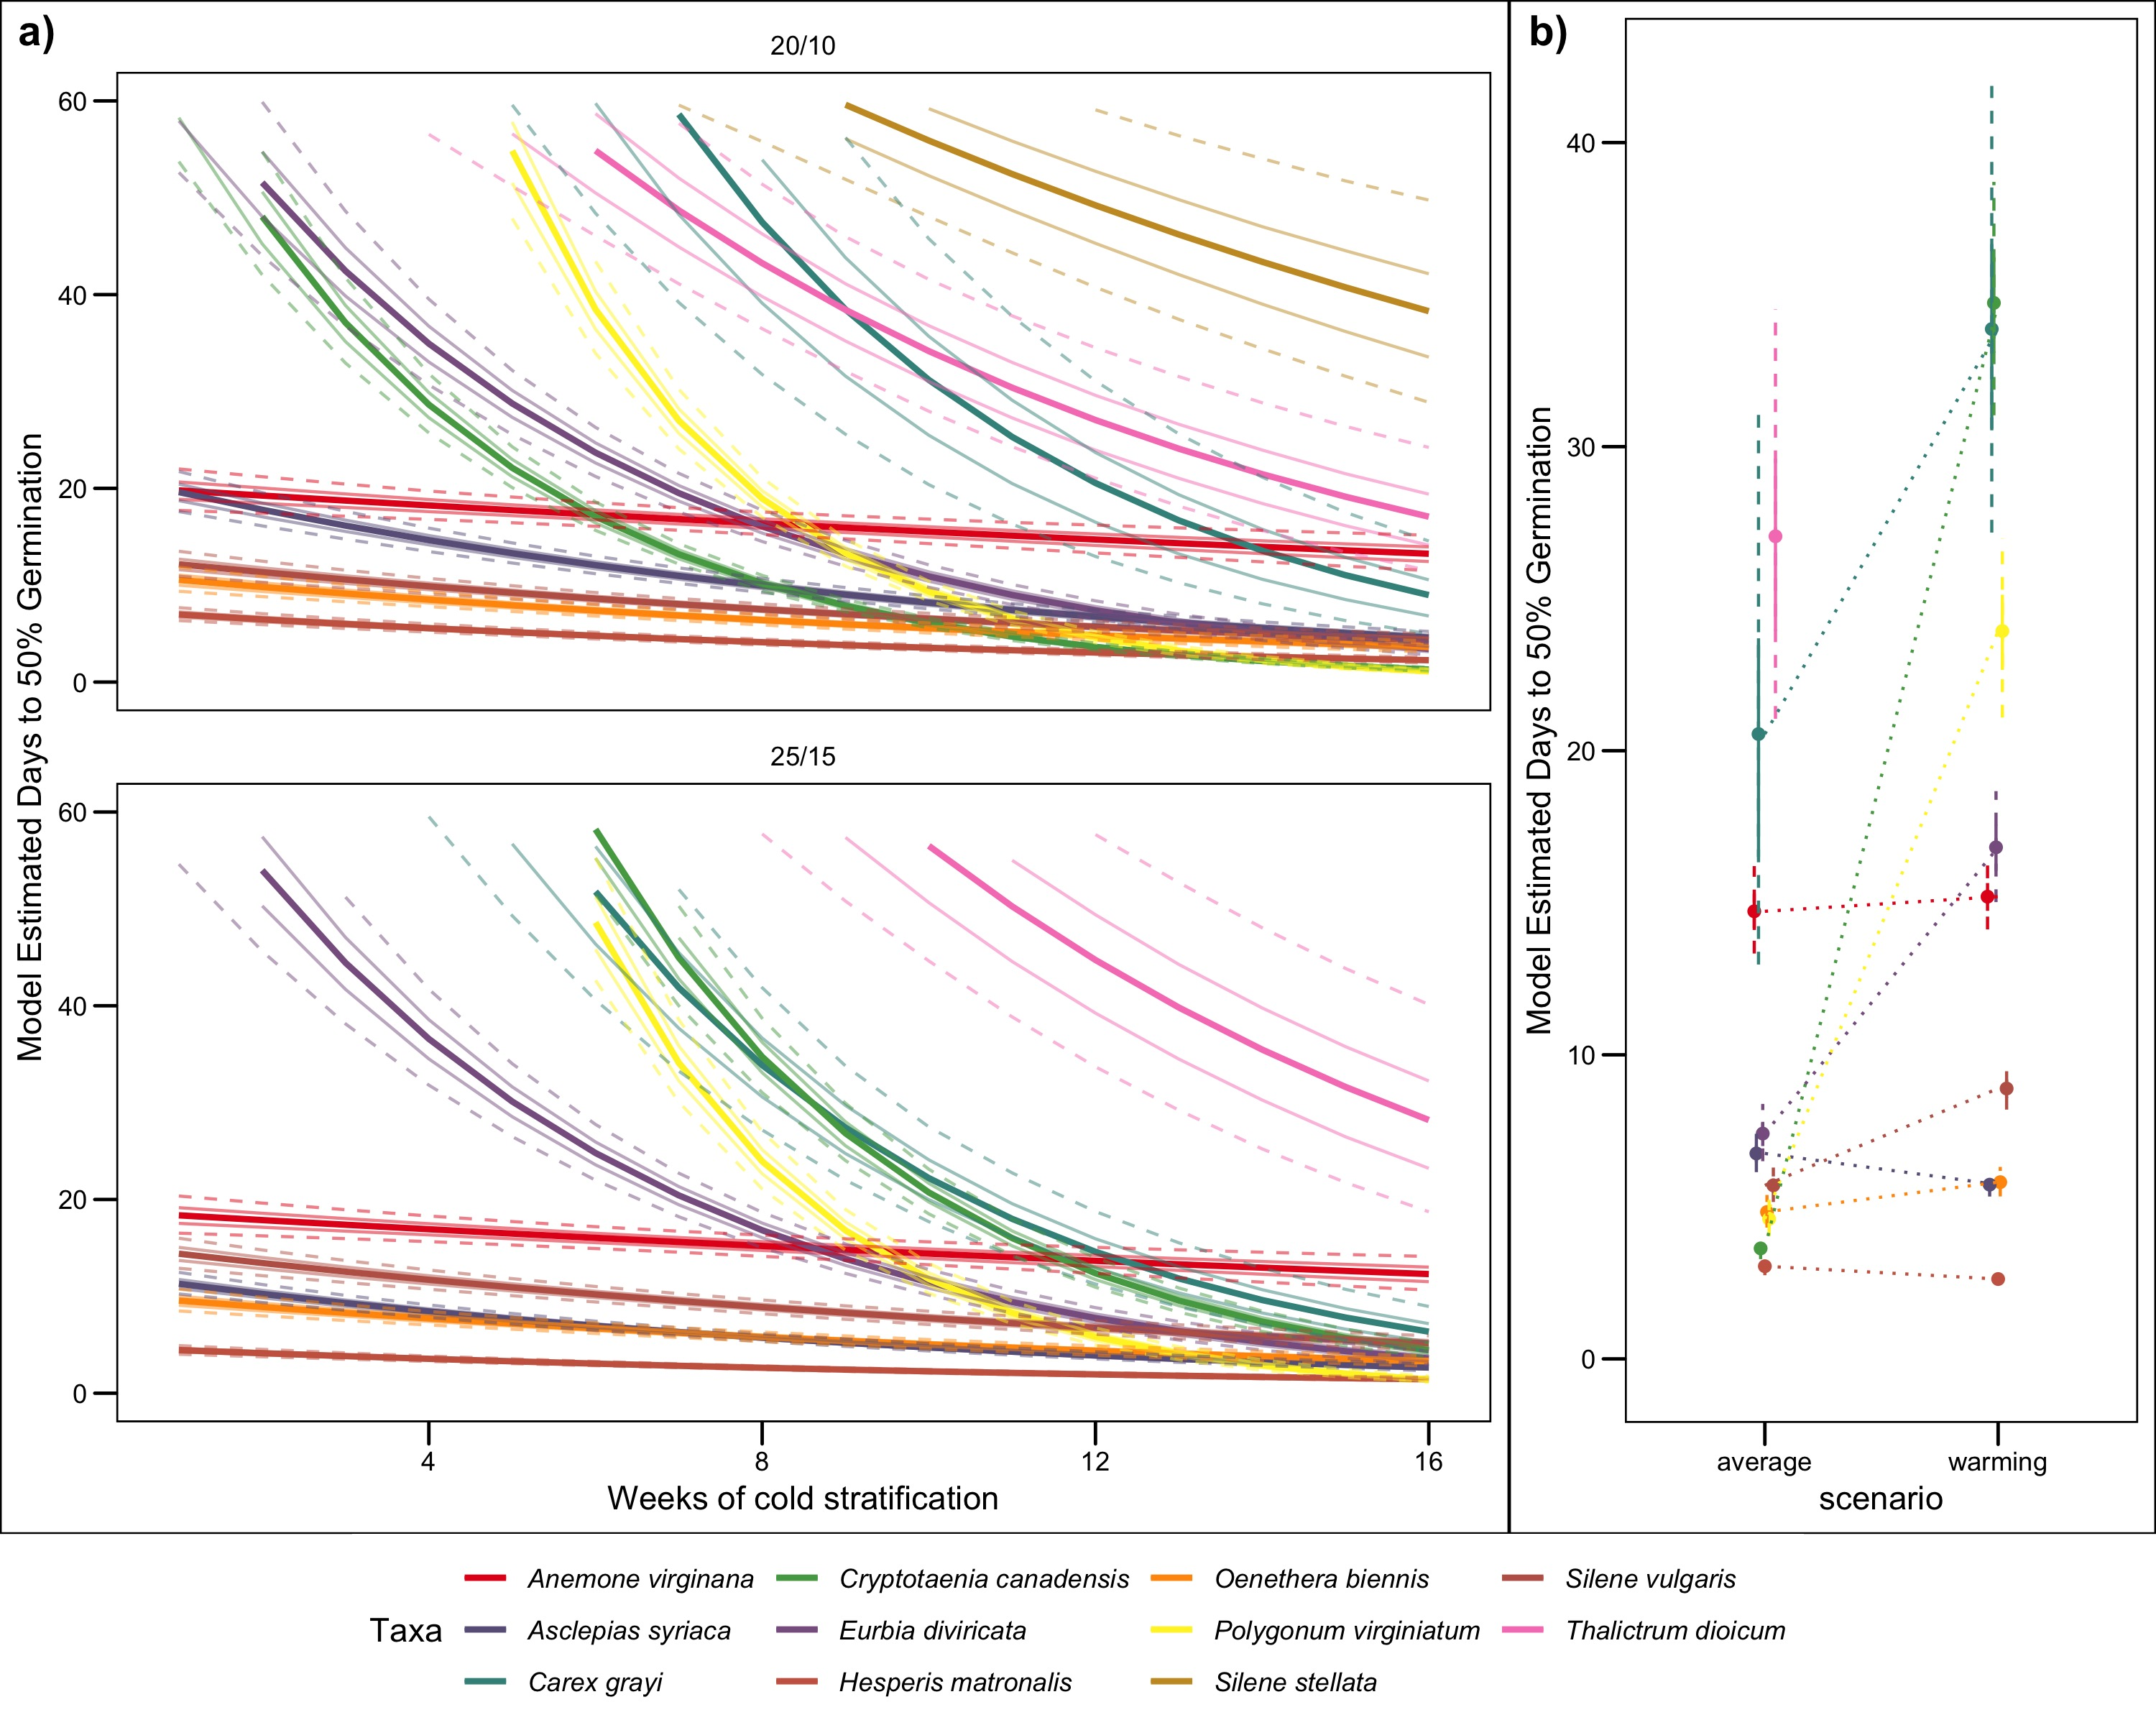
\includegraphics[width=\textwidth]{..//figures/AFTplots.jpeg} 
    \caption{} 
    \label{fig:AFT}
\end{figure}

\section*{Tables}
\begin{landscape}
\begin{sidewaystable}

\begin{kframe}


{\ttfamily\noindent\itshape\color{messagecolor}{\#\# Registered S3 method overwritten by 'xts':\\\#\#\ \  method\ \ \ \  from\\\#\#\ \  as.zoo.xts zoo}}\end{kframe}% latex table generated in R 3.6.2 by xtable 1.8-4 package
% Mon Dec 21 13:32:17 2020
\scalebox{0.8}{
\begin{tabular}{rllllllllllll}
  \hline
 & Taxa & Hesperis matronalis & Silene vulgaris & Oenethera biennis & Asclepias syriaca & Silene stellata & Eurbia diviricata & Anemone virginana & Cryptotaenia canadensis & Carex grayi & Thalictrum dioicum & Polygonum virginiatum \\ 
  \hline
1 & Hesperis matronalis &  &  &  &  &  &  &  &  &  &  &  \\ 
  2 & Silene vulgaris & 3.6 &  &  &  &  &  &  &  &  &  &  \\ 
  3 & Oenethera biennis & 1.4 & -2.2 &  &  &  &  &  &  &  &  &  \\ 
  4 & Asclepias syriaca & -0.6 & -4.2 & -2 &  &  &  &  &  &  &  &  \\ 
  5 & Silene stellata & 124.6 & 121 & 123.2 & 125.2 &  &  &  &  &  &  &  \\ 
  6 & Eurbia diviricata & 9.8 & 6.2 & 8.4 & 10.4 & -114.7 &  &  &  &  &  &  \\ 
  7 & Anemone virginana & 0.9 & -2.7 & -0.5 & 1.5 & -123.7 & -8.9 &  &  &  &  &  \\ 
  8 & Cryptotaenia canadensis & 31.5 & 27.9 & 30.1 & 32.1 & -93.1 & 21.7 & 30.6 &  &  &  &  \\ 
  9 & Carex grayi & 13.7 & 10.1 & 12.3 & 14.3 & -110.8 & 3.9 & 12.8 & -17.8 &  &  &  \\ 
  10 & Thalictrum dioicum & 44.9 & 41.3 & 43.5 & 45.5 & -79.7 & 35.1 & 44 & 13.4 & 31.2 &  &  \\ 
  11 & Polygonum virginiatum & 19.8 & 16.1 & 18.3 & 20.4 & -104.8 & 9.9 & 18.9 & -11.8 & 6 & -25.2 &  \\ 
   \hline
\end{tabular}
}

\end{sidewaystable}
\end{landscape}

\end{document}
